\documentclass{article}
\usepackage[T1]{fontenc}
\usepackage{lmodern}
\usepackage{graphicx}
\usepackage{amsmath,amssymb}
\usepackage[a4paper,margin=2cm]{geometry}
\usepackage[absolute,overlay]{textpos}
\setlength{\TPHorizModule}{1mm}
\setlength{\TPVertModule}{1mm}
\usepackage[indonesian]{babel}
\usepackage{hyperref}
\setlength{\emergencystretch}{2em}
% unit: Halaman 19

\begin{document}

% === Halaman 19 (python/native) ===

Ri-1

32 bit

E(Ri-1)

Ekspansi menjadi 48 bit

48 bit



Ki

48 bit

A

K

R

E

i

i

=



−)

(

1

S1

S8

...

B

Matriks substitusi

32 bit

48 bit

P(B)

32 bit

Gambar 5. Diagram komputasi fungsi f:

19

f

% deskripsi: gambar native xref 109
\noindent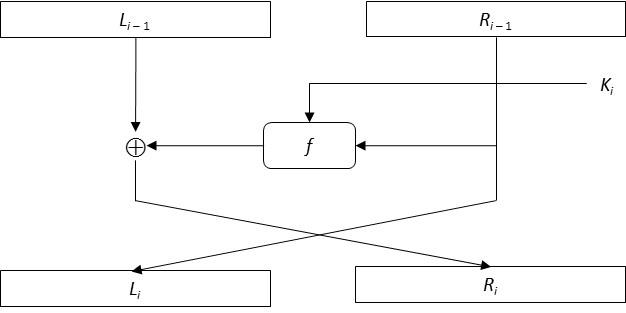
\includegraphics[width=0.85\textwidth]{../../images/python/page_019_img_01.jpeg}

\end{document}
